\documentclass[journal,onecolumn]{IEEEtran}

% correct bad hyphenation here
%\hyphenation{op-tical net-works semi-conduc-tor}

\usepackage{graphicx}
\usepackage{float}
\usepackage{booktabs}
\usepackage{caption}
\usepackage{subcaption}
\graphicspath{{Images/}}

\setlength{\parskip}{1em} 

\begin{document}
%
% paper title
% Titles are generally capitalized except for words such as a, an, and, as,
% at, but, by, for, in, nor, of, on, or, the, to and up, which are usually
% not capitalized unless they are the first or last word of the title.
% Linebreaks \\ can be used within to get better formatting as desired.
% Do not put math or special symbols in the title.
\title{EECE 571 Course Project: Modulation\\ Classification Using Neural Networks}
%
%
% author names and IEEE memberships
% note positions of commas and nonbreaking spaces ( ~ ) LaTeX will not break
% a structure at a ~ so this keeps an author's name from being broken across
% two lines.
% use \thanks{} to gain access to the first footnote area
% a separate \thanks must be used for each paragraph as LaTeX2e's \thanks
% was not built to handle multiple paragraphs
%

\author{Akshay~Viswakumar (Student\# 32971665), \\Department of Electrical \& Computer Engineering, \\The University of Birtish Columbia
}

% note the % following the last \IEEEmembership and also \thanks - 
% these prevent an unwanted space from occurring between the last author name
% and the end of the author line. i.e., if you had this:
% 
% \author{....lastname \thanks{...} \thanks{...} }
%                     ^------------^------------^----Do not want these spaces!
%
% a space would be appended to the last name and could cause every name on that
% line to be shifted left slightly. This is one of those "LaTeX things". For
% instance, "\textbf{A} \textbf{B}" will typeset as "A B" not "AB". To get
% "AB" then you have to do: "\textbf{A}\textbf{B}"
% \thanks is no different in this regard, so shield the last } of each \thanks
% that ends a line with a % and do not let a space in before the next \thanks.
% Spaces after \IEEEmembership other than the last one are OK (and needed) as
% you are supposed to have spaces between the names. For what it is worth,
% this is a minor point as most people would not even notice if the said evil
% space somehow managed to creep in.

% The paper headers
\markboth{Project Submission for EECE 571M Term 2, 2019 / 2020}%
{Viswakumar (\# 32971665) \: Modulation Classification Using Neural Networks}
% The only time the second header will appear is for the odd numbered pages
% after the title page when using the twoside option.
% 
% *** Note that you probably will NOT want to include the author's ***
% *** name in the headers of peer review papers.                   ***
% You can use \ifCLASSOPTIONpeerreview for conditional compilation here if
% you desire.




% If you want to put a publisher's ID mark on the page you can do it like
% this:
%\IEEEpubid{0000--0000/00\$00.00~\copyright~2015 IEEE}
% Remember, if you use this you must call \IEEEpubidadjcol in the second
% column for its text to clear the IEEEpubid mark.



% use for special paper notices
%\IEEEspecialpapernotice{(Invited Paper)}

% use for special paper notices
%\IEEEspecialpapernotice{(Invited Paper)}




% make the title area
\maketitle

% As a general rule, do not put math, special symbols or citations
% in the abstract or keywords.
%\begin{abstract}
%The abstract goes here.
%\end{abstract}

% Note that keywords are not normally used for peerreview papers.
%\begin{IEEEkeywords}
%IEEE, IEEEtran, journal, \LaTeX, paper, template.
%\end{IEEEkeywords}

% For peer review papers, you can put extra information on the cover
% page as needed:
% \ifCLASSOPTIONpeerreview
% \begin{center} \bfseries EDICS Category: 3-BBND \end{center}
% \fi
%
% For peerreview papers, this IEEEtran command inserts a page break and
% creates the second title. It will be ignored for other modes.
\IEEEpeerreviewmaketitle


\section{Introduction}
% The very first letter is a 2 line initial drop letter followed
% by the rest of the first word in caps.
% 
% form to use if the first word consists of a single letter:
% \IEEEPARstart{A}{demo} file is ....
% 
% form to use if you need the single drop letter followed by
% normal text (unknown if ever used by the IEEE):
% \IEEEPARstart{A}{}demo file is ....
% 
% Some journals put the first two words in caps:
% \IEEEPARstart{T}{his demo} file is ....
% 
% Here we have the typical use of a "T" for an initial drop letter
% and "HIS" in caps to complete the first word.
\IEEEPARstart{T}{he} goal of Automatic Modulation Classification (AMC) is to be able to infer the type of modulation technique by observing samples of received signals. This is a pattern recognition task and a good classifier would need to base its decision solely on key features extracted from the received signal and no other prior knowledge. A good classifier must also be robust and capable of making inferences from real world signals which are subject to degradation due to effects of channel fading and noise.

An intuitive choice of a solution to the problem of AMC would be to design a classifier that is trained using supervised learning techniques. This notion is intuitive because:
(1)	Supervised learning techniques continue to demonstrate time and again, their superiority over conventional algorithms and techniques for popular classification problems, given enough labeled training data. 
(2)	At present, there is no dearth of labeled training data for this problem with plenty of datasets which may be sampled from actual over-the-air recordings or synthetically generated using tools like GNU Radio. The dataset that has been provided for this project, “RADIOML 2016.10A” is a synthetic dataset (with simulated effects of channel conditions) that was created and made available to the community by DEEPSIG \cite{rmlDset}.

The goal of this project was to design an Artificial Neural Network (ANN) solution and a Convolutional Neural Network (CNN) solution to the AMC problem. This report documents the work carried out in pursuit of the aforementioned goal.  The remainder of this report is organised in the following manner. Section 2 is an analysis of the available dataset and a discussion of choices (common to both solutions) made to pre-process and segment the data. Section 3 and Section 4 deal with the ANN and CNN solutions respectively. Each of these sections start with a small background sub-section, a discussion of related work followed by design choices, observations and results. Finally, both solutions are compared in Section 5. The choice to include related work and background within the sections they are discussed in may be a little unconventional, but I believe this will greatly improve the way this report reads.

% You must have at least 2 lines in the paragraph with the drop letter
% (should never be an issue)

%\hfill mds
 
%\hfill August 26, 2015
% needed in second column of first page if using \IEEEpubid
%\IEEEpubidadjcol

\section{RADIOML Data}

\subsection{Description of Data}

The dataset consists of 220,000 labelled signals. Signal samples are split and their real and imaginary components are stored separately. In this way, each signal is a 2x128 array representing 128 $\mu$s of a received waveform sampled at $10^{6}$ samples/second. Each signal is labelled based on both the modulation technique as well as the signal-to-noise ratio (SNR) value. There are 11 different classes based on modulation techniques  (8PSK, AM-DSB, AM-SSB, BPSK, CPFSK, GFSK, PAM4, QAM16, QAM64, QPSK, WBFM). There are 20 different classes based on the SNR (-20, -18, -16, -14, -12, -10, -8, -6, -4, -2, 0, 2, 4, 6, 8, 10, 12, 14, 16, 18).

\subsection{Pre-Processing}

The dataset is available as a pickle file that stores a python data structure in a serialized manner. Data from the pickle file were loaded into Numpy Arrays. The loaded label data consisted of binary strings which aren't otherwise meaningful to a neural network. The modulation labels were converted into on-hot encoded vectors where each vector was 1x11 and each bit represented one of the 11 modulation techniques.

Normalization is carried out on feature vectors before they are fed into the respective neural networks. This will be discussed in subsequent sections since the kind of feature vectors are different between the ANN and CNN networks.

\subsection{Partitioning via Stratified Sampling}

The available dataset was split in half to form training and testing datasets consisting of 110,000 samples each. The training set was then partitioned once again where 90\% of the samples went on to form the actual Training set and 10\% of the samples used to form a Validation set.

Each partition of the data set was formed in a way that there was adequate representation from all modulation and SNR classes. This was to make sure that the neural network could observe nearly the same number of samples from all possible classes and that there wouldn't be any over-representation or bias for one class or the other. Refer to Figure 1 and Figure 2 which display the histograms of the partitioned dataset based on SNR and Modulation Techniques. This sort of Stratified Sampling \cite{stratSamp} was possible because the original dataset has been designed in such a way that there is equal representation from all classes.

\begin{figure}[h]
	\centering
	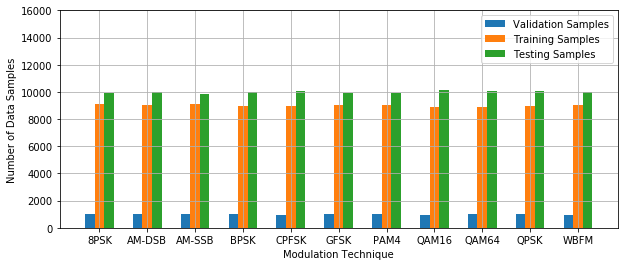
\includegraphics[scale=0.6]{stratSampleModTech}
	\caption{Histogram of Partitioned Data, grouped by Modulation Technique}
	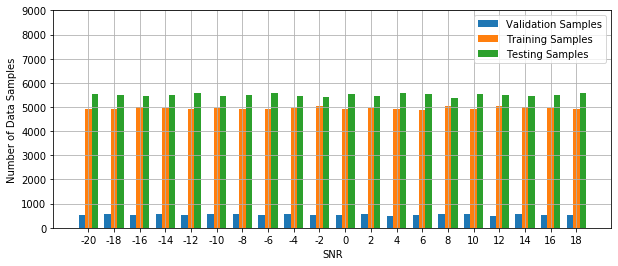
\includegraphics[scale=0.6]{stratSampleSNR}
	\caption{Histogram of Partitioned Data, grouped by SNR}		
\end{figure}

The Keras framework is able to reserve a portion of the training set for validation purposes at the time of training. However, the source of entropy for this is not within the user's control. Data was manually partitioned (using seeded pseudo-random number generators) in an effort to ensure that datasets stayed the same across different tests.

\section{Artificial Neural Network (ANN) Solution}

\subsection{Background}

\subsection{Related Work}

\subsection{Network Design}

\subsection{Observations}

\subsection{Results}

\section{Convolutional Neural Network (CNN) Solution}

\subsection{Background}

CNNs take inspiration from the mammalian visual system. In particular, the way how the brain processes visual information hierarchically often starting with simple structures such as oriented edges \cite{catEye}. In the late 70s, Fukushima applied this idea to create the Neocognitron \cite{neocognitron}, a predecessor to CNNs, which was built to detect handwritten characters. The Neocognitron introduced the notion of a convolutional layer which was a spatially invariant filter that could be used to detect features irrespective of location in an image. The coefficients of the convolutional filter still had to be trained via some supervised learning algorithm. Fast forward to 1998, when LeCun et al \cite{lenet5} applied error backpropagation to train convolutional filter coefficients leading to the birth of CNNs as we now know them.

While CNNs, like UNet \cite{unet} may be built using convolutional layers alone, they often make use of fully connected neurons when performing classification. In a CNN designed for classification, the initial convolutional layers essentially perform feature extraction.

\subsection{Related Work}

CNNs are commonly used in problems where the input data consist of images. However, they can be useful in any task where data has features that are spatially relevant such as in the case of text classification or speech recognition. Along the same lines, CNNs can be useful in AMC where the input data is made up of finite number of symbols that are unique for a given modulation scheme. 

There are a lot of papers that present the solutions to the AMC problem. Each paper proposes one type of network design or the other and claims it to be best suited to the task. However, there’s often nothing more than empirical evidence to back their claims. This sort of situation is also commonplace in other domains, computer vision for instance, where neural networks are rampant.

That said, a number of recent publications were reviewed in an effort to identify “best-practices” that have proven helpful for designing a CNN for AMC. O’Shea et al \cite{cnn2} achieve reasonably good performance on the RADIOML 2016.10A dataset with two CNN based networks. These networks are able to get over 10\% accuracy for the lowest SNRs and above 80\% accuracy for higher SNRs. Both networks consist of two convolutional layers and a fully connected layer (excluding the final classification layer). They differ only in that one design has more filters in the convolutional layers that the other. Both networks make use of the Adam optimizer as well as dropout for regularization. A lot of details are left to interpretation. Ramjee et al \cite{cnn1} make use of a deeper CNN design with four convolutional layers based on the more complex CNN proposed in \cite{cnn2}. While they report a higher accuracy at high SNRs (over 80\% at 18dB), their network does not do well at the lower SNRs. 

Lee and colleagues propose an interesting solution in \cite{featImage} wherein they first extract a number of statistical features (such as higher order cumulants) which are then used to compose a “feature image” which is then fed into a CNN. Their claim is that feature images are distinct for a given modulation technique. The results they report indicate an improvement in the accuracies at high SNRs (nearly 100\% over 4dB). The performance at lower SNRs are not very remarkable.

In \cite{ddriven}, Wang and Yang highlight a problem that I have observed during my experiments. It is difficult for most CNNs that operate on the input signal in rectangular form to differentiate between QAM-16 and QAM-64 modulation even at the highest SNR. The authors use an additional CNN used exclusively to differentiate between QAM-16 and QAM-64. This secondary network uses constellation diagrams as input.

\subsection{Network Design}

\begin{table}
\centering
\caption{Design of CNN-AV}
\label{tab:my-table}
\begin{tabular}{@{}cccc@{}}
\toprule
Layer & Layer Type  & Description                               & Activation \\ \midrule
1     & Convolution & 512 Filters, Size = (1,3), Stride = (1,1) & ReLU       \\
2     & MaxPooling  & Window = (1,2), Stride = (1,2)            & -          \\
3     & Dropout     & Dropout Rate = 0.5                        & -          \\
4     & Convolution & 256 Filters, Size = (1,3), Stride = (1,1) & ReLu       \\
5     & MaxPooling  & Window = (1,2), Stride = (1,2)            & -          \\
6     & Dropout     & Dropout Rate = 0.5                        & -          \\
7     & Convolution & 128 Filters, Size = (1,3), Stride = (1,1) & ReLu       \\
8     & MaxPooling  & Window = (1,2), Stride = (1,2)            & -          \\
9     & Dropout     & Dropout Rate = 0.5                        & -          \\
10    & Convolution & 64 Filters, Size = (1,3), Stride = (1,1)  & ReLu       \\
11    & MaxPooling  & Window = (1,2), Stride = (1,2)            & -          \\
12    & Dropout     & Dropout Rate = 0.5                        & -          \\
13    & Dense       & Units = 128                               & ReLu       \\
14    & Dense       & Units = 11                                & SoftMax    \\ \bottomrule
\end{tabular}
\end{table}

\subsection{Observations}

\begin{figure*}[h]
    \centering
    \begin{subfigure}[b]{0.4\textwidth}
        \centering
        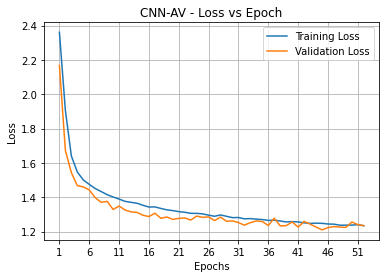
\includegraphics[scale=0.5]{cnnavPerf}
        \caption{Training Performance}
    \end{subfigure}%
    ~ 
    \begin{subfigure}[b]{0.4\textwidth}
        \centering
        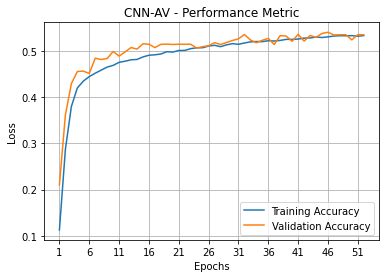
\includegraphics[scale=0.5]{cnnavPerfMet}
        \caption{Performance Metric}
    \end{subfigure}
    \caption{CNN-AV - Accuracy and Loss During Training}
\end{figure*}

Testing

\begin{figure*}[h]
    \centering
    \begin{subfigure}[b]{0.5\textwidth}
        \centering
        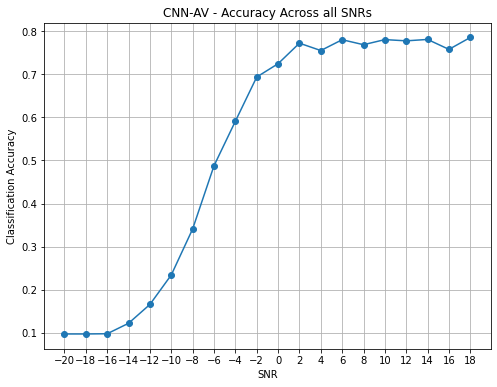
\includegraphics[scale=0.5]{cnnACCSNR}
        \caption{Performance Metric}
    \end{subfigure}%
    ~ 
    \begin{subfigure}[b]{0.5\textwidth}
        \centering
        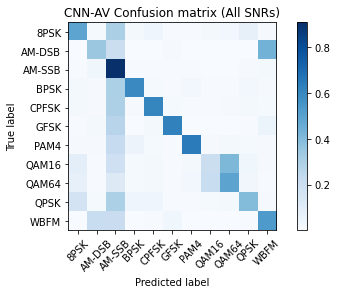
\includegraphics[scale=0.7]{cnnoverallConfMat}
        \caption{Confusion Matrix}
    \end{subfigure}
    \caption{Performance of CNN-AV on Test Data}
\end{figure*}

CONF MATRIX

\begin{figure}[!ht]
   \centering
   \subfloat[][]{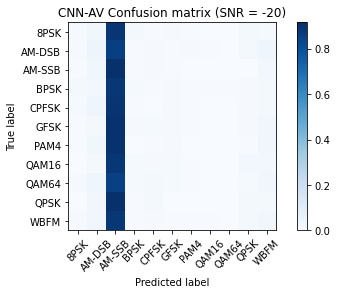
\includegraphics[width=.4\textwidth]{-20}}\quad
   \subfloat[][]{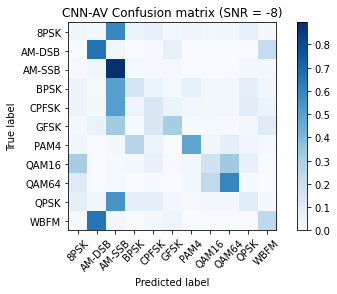
\includegraphics[width=.4\textwidth]{-8}}\\
   \subfloat[][]{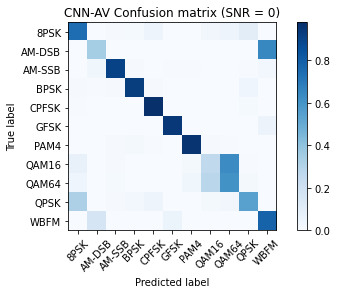
\includegraphics[width=.4\textwidth]{0}}\quad
   \subfloat[][]{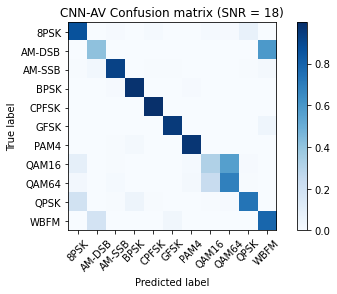
\includegraphics[width=.4\textwidth]{18}}
   \caption{CNN-AV Confusion Matrix at Different SNRs}
   \label{fig:sub1}
\end{figure}

\subsection{Results}

\section{Conclusion}

% use section* for acknowledgment
%\section*{Acknowledgment}

% Can use something like this to put references on a page
% by themselves when using endfloat and the captionsoff option.
\ifCLASSOPTIONcaptionsoff
  \newpage
\fi



% trigger a \newpage just before the given reference
% number - used to balance the columns on the last page
% adjust value as needed - may need to be readjusted if
% the document is modified later
%\IEEEtriggeratref{8}
% The "triggered" command can be changed if desired:
%\IEEEtriggercmd{\enlargethispage{-5in}}

% references section

% can use a bibliography generated by BibTeX as a .bbl file
% BibTeX documentation can be easily obtained at:
% http://mirror.ctan.org/biblio/bibtex/contrib/doc/
% The IEEEtran BibTeX style support page is at:
% http://www.michaelshell.org/tex/ieeetran/bibtex/
%\bibliographystyle{IEEEtran}
% argument is your BibTeX string definitions and bibliography database(s)
%\bibliography{IEEEabrv,../bib/paper}
%
% <OR> manually copy in the resultant .bbl file
% set second argument of \begin to the number of references
% (used to reserve space for the reference number labels box)
\bibliographystyle{IEEEtran}
\bibliography{eece571MProjectReferences}

% biography section
% 
% If you have an EPS/PDF photo (graphicx package needed) extra braces are
% needed around the contents of the optional argument to biography to prevent
% the LaTeX parser from getting confused when it sees the complicated
% \includegraphics command within an optional argument. (You could create
% your own custom macro containing the \includegraphics command to make things
% simpler here.)
%\begin{IEEEbiography}[{\includegraphics[width=1in,height=1.25in,clip,keepaspectratio]{mshell}}]{Michael Shell}
% or if you just want to reserve a space for a photo:

%\vfill

% Can be used to pull up biographies so that the bottom of the last one
% is flush with the other column.
%\enlargethispage{-5in}



% that's all folks
\end{document}


